\providecommand{\main}{..} 
\documentclass[\main/boa.tex]{subfiles}

\begin{document}

\section{Show Me Your Model}


\begin{minipage}{0.915\textwidth}
	\centering
  {\bf \LARGE \index[a]{Biecek Przemysław} Przemysław Biecek}
\end{minipage}

\begin{affiliations}
\begin{minipage}{0.915\textwidth}
\centering
\large MI$^{2}$  \\[1pt]
Kontakt: \href{mailto:przemyslaw.biecek@gmail.com}{\nolinkurl{przemyslaw.biecek@gmail.com}}\\
\end{minipage}
\end{affiliations}


Gramatyka grafiki (Wilkinson, Leland. 2006. The Grammar of Graphics) i jej implementacje (Wickham, Hadley. 2009. Ggplot2: Elegant Graphics for Data Analysis) zmieniły sposób w jaki myślimy o wizualizacji danych. Podobna rewolucja czeka wizualizacje modeli statystycznych. Podczas referatu przedstawię różne istniejące narzędzia do prezentacji modeli statystycznych (rms, forestmodel and regtools, survminer, \break ggRandomForests, factoextra, factorMerger) oraz zderzę je z jednolitym podejściem do przetwarzania modeli prezentowanym przez pakiet broom (Robinson, David. 2017. Broom: Convert Statistical Analysis Objects into Tidy Data Frames). Prezentacje zakończy zbiór doświadczeń dotyczących wizualizacji struktury modelu (Wickham, Hadley, Dianne Cook, and Heike Hofmann. 2015. Visualizing Statistical Models: Removing the Blindfold. Statistical Analysis) 

\bio  
\begin{wrapfigure}{r}{100px}
    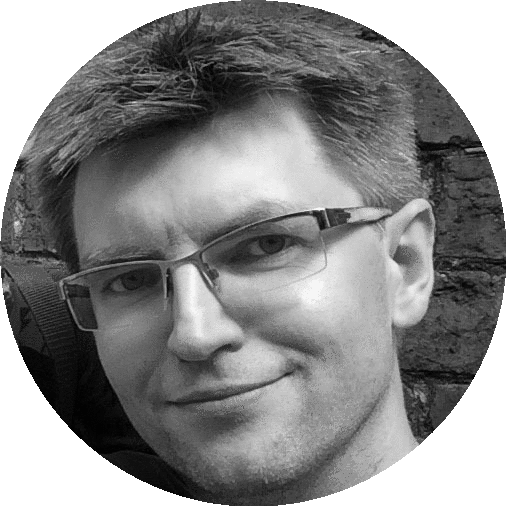
\includegraphics[width=100px]{img/guests/czarno_biale/pbiecek.png}
\end{wrapfigure} 
Dr hab. inż. Przemysław Biecek, prof. PW od kilkunastu lat pracuje nad metodami modelowania wysokowymiarowych danych dużego wolumenu. W roku 2003 ukończył studia magisterskie w specjalnościach “Inżynieria Oprogramowania” i “Statystyka Matematyczna” na Politechnice Wrocławskiej, w roku 2007 obronił doktorat, a w roku 2013 obronił habilitację w obszarze Statystyka Medyczna.

Aktywnie współpracuje z biznesem, wybrane większe projekty: z działem badawczym firmy Netezza przy zanurzaniu natywnego rozproszonego przetwarzania danych wewnątrz hurtowni danych; z~działem badawczym IBM przy analizie i wizualizacji danych z sieci społecznościach; z działem badawczym iQor Polska przy profilowaniu zachowań konsumenckich; z działem badawczym OECD przy badaniu rozkładu kapitału naukowego międzynarodowej młodzieży.

W pracy naukowej interesuje się technikami modelowania wysokowymiarowych danych (testowania zbioru hipotez oraz wyboru modelu), jak i wizualizacją danych oraz aplikacjami w medycynie i genomice. Jest autorem lub współautorem 55 publikacji z listy JCR. Wiele z ostatnich publikacji jest poświęconych analizie danych onkologicznych.

Jest autorem trzech popularnych podręczników akademickich poświęconych programowi R (Przewodnik po programie R, GiS 2017), analizie danych (Modele liniowe i mieszane, PWN 2015) i wizualizacji danych (Odkrywać! Ujawniać! Objaśniać! 2016). W ramach działalności popularyzującej naukę współorganizuje liczne konferencje i spotkania poświęcone programowi R (Why R? 2017, UseR 2017, eRum 2016, SER 2014-2017, WZUR 2008-2012). 

Pracuje również nad projektem pozaakademickiej edukacji statystycznej (projekt Beta i Bit).

\end{document}
